% !TEX program = lualatex
\documentclass[10pt]{beamer}

\usetheme[progressbar=frametitle]{metropolis}
\usepackage{appendixnumberbeamer}

\usepackage{graphicx}
\usepackage{booktabs}
\usepackage{tabularx}
\usepackage{colortbl}
\usepackage[scale=2]{ccicons}

\usepackage{braket}

\usepackage{pgfplots}
\usepgfplotslibrary{dateplot,fillbetween}
\pgfplotsset{compat=1.18}
\usepackage[font=scriptsize,labelfont=bf]{caption}

\usepackage{listings}

\usepackage{tikz}
\usetikzlibrary{fit,shapes,positioning,calc,shapes.geometric,backgrounds}
\colorlet{tempGray}{gray!80!cyan}
\colorlet{lightgray}{tempGray!60!white}
\colorlet{orange}{red!30!yellow}
\colorlet{lightorange}{orange!60!white}
\colorlet{darkGreen}{green!80!black}
\colorlet{paleGreen}{darkGreen!30!white}

\usepackage{hyperref}
\usepackage{xspace}
\newcommand{\themename}{\textbf{\textsc{metropolis}}\xspace}

\def\code#1{\texttt{#1}}
\newcommand{\lighthline}{\arrayrulecolor{gray!35}\hline\arrayrulecolor{black}}

\lstset{
    language=Python,
    basicstyle=\ttfamily\tiny,
    keywordstyle=\color{blue!80!black},
    commentstyle=\color{gray},
    frame=single,
    breaklines=true,
    showstringspaces=false,
    aboveskip=2pt,
    belowskip=2pt,
}

\title{NetSquid for Quantum Networks}
\subtitle{Capabilities, Bottlenecks and Lessons}
\author{Linus Kelsey}
\date{29 Jul 2026}
\institute{UCL Physics \& Astronomy}

\begin{document}

\maketitle

% ── WHY SIMULATE ─────────────────────────────────────────────────────────────
\begin{frame}{Why Simulate Quantum Networks?}
  \textbf{Bridging the gap from device physics to network deployment}

    \begin{center}
    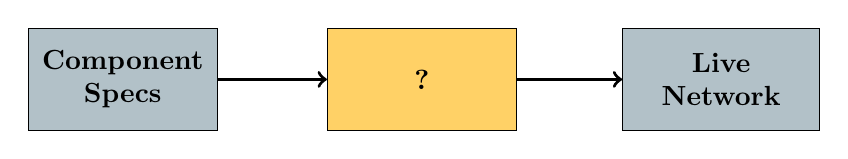
\begin{tikzpicture}
        \node[draw, fill=lightgray, minimum width=2.4cm, minimum height=1.3cm, align=center] (dev) at (0,0)
          {\textbf{Component}\\\textbf{Specs}};
        \node[draw, fill=lightorange, minimum width=2.4cm, minimum height=1.3cm, align=center] (sim) at (3.8,0)
            {\textbf{?}};
        \node[draw, fill=lightgray, minimum width=2.5cm, minimum height=1.3cm, align=center] (sys) at (7.6,0)
          {\textbf{Live}\\\textbf{Network}};
        \draw[->, very thick] (dev) -- (sim);
        \draw[->, very thick] (sim) -- (sys);
    \end{tikzpicture}
    \end{center}

    Immediate deployment = expensive, slow, unpredictable.
    \begin{itemize}
        \item Analytical models: closed-form but fixed
        \item Computational: arbitrary protocols and parameters, immediate reconfigurability (Bel \textit{et al.}, 2024)
    \end{itemize}

    \vspace{0.2cm}
    Enter... NetSquid (Coopmans \textit{et al.}, 2021)!
\end{frame}

% ── WHAT IS NETSQUID ──────────────────────────────────────────────────────────
\begin{frame}{NetSquid: Discrete-Event Simulator}
    \begin{columns}[T]
        \begin{column}{0.50\textwidth}
            \textbf{Design}
            \begin{itemize}
                \item Quantum events on bespoke Cython DES layer - PyDynAA
                \item Three core networking abstractions: \texttt{Component}, \texttt{Node}, \texttt{Protocol}
                \item Custom devices, models and behaviours
            \end{itemize}
        \end{column}
        \begin{column}{0.48\textwidth}
          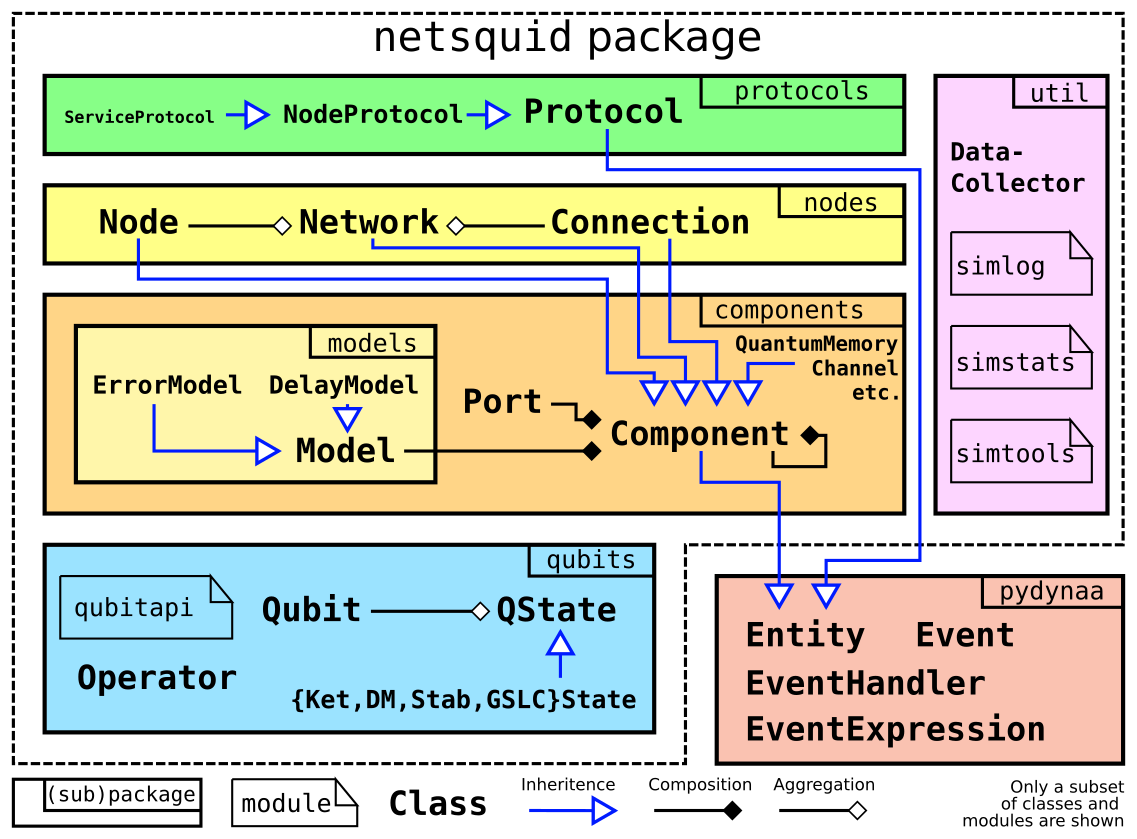
\includegraphics[width=\linewidth]{artefacts/img/netsquidstack_detailed.png}
          \vspace{0.05cm}
          \scriptsize NetSquid architecture - per \href{https://netsquid.org}{netsquid.org}
        \end{column}
    \end{columns}
\end{frame}

% ── BRIDGE: CONNECTING DEVICE PHYSICS TO NETWORK MODELLING ──────────────────
\begin{frame}{Bridging Device Physics to Network Modelling}
    \textbf{Measurements drive simulations, informing network optimisation}

    \vspace{0.2cm}
    \begin{center}
    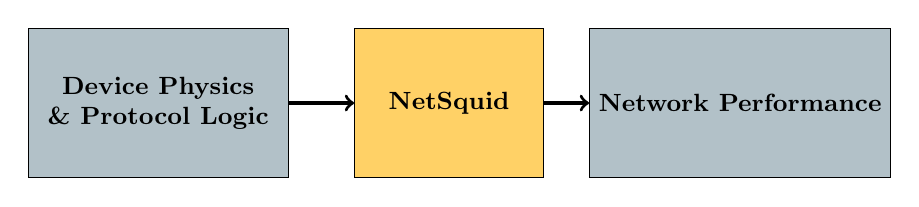
\begin{tikzpicture}[every node/.style={font=\small}, scale=0.88]
        % Device characterization (left)
        \node[draw, fill=lightgray, minimum width=3.3cm, minimum height=1.9cm, align=center] (dev) at (0,0)
            {\textbf{Device Physics}\\
            \textbf{\& Protocol Logic}};

        % NetSquid (center)
        \node[draw, fill=lightorange, minimum width=2.4cm, minimum height=1.9cm, align=center] (sim) at (4.2,0)
            {\textbf{NetSquid}};

        % Network design (right)
        \node[draw, fill=lightgray, minimum width=3.3cm, minimum height=1.9cm, align=center] (net) at (8.4,0)
            {\textbf{Network Performance}};
        
        \draw[->, very thick] (dev) -- (sim);
        \draw[->, very thick] (sim) -- (net);
    \end{tikzpicture}
    \end{center}

    \vspace{0.25cm}
    \begin{columns}[T]
        \begin{column}{0.48\textwidth}
            \small \textbf{What you provide}
            \begin{itemize}\small
                \item Measured device parameters
                \item Noise models, logic
                \item Physical constraints e.g. QBER
            \end{itemize}
        \end{column}
        \begin{column}{0.48\textwidth}
            \small \textbf{What you gain}
            \begin{itemize}\small
                \item Network feasibility
                \item Architecture optimisation
                \item Device parameter sensitivity
            \end{itemize}
        \end{column}
    \end{columns}
\end{frame}

% ── RUNNING EXAMPLE ───────────────────────────────────────────────────────────
\begin{frame}{Running Example: BB84 and MDI-QKD}
    \small Basis of MSc research, used throughout to ground NetSquid discussion

    \vspace{0.8cm}
    \begin{columns}[T]
        \begin{column}{0.47\textwidth}
            \textbf{BB84} \textnormal{\scriptsize (Bennett \& Brassard, 1984)}
            \begin{center}
            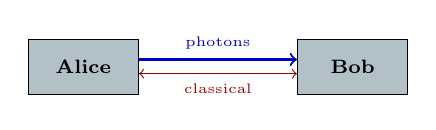
\begin{tikzpicture}[every node/.style={font=\scriptsize}, scale=0.9]
                \node[draw, fill=lightgray, minimum width=1.4cm, minimum height=0.7cm, align=center] (a) at (0,0) {\textbf{Alice}};
                \node[draw, fill=lightgray, minimum width=1.4cm, minimum height=0.7cm, align=center] (b) at (3.8,0) {\textbf{Bob}};
                \draw[->, blue!80!black, thick] ([yshift=0.1cm]a.east) -- node[above]{\tiny photons} ([yshift=0.1cm]b.west);
                \draw[<->, red!60!black] ([yshift=-0.1cm]a.east) -- node[below]{\tiny classical} ([yshift=-0.1cm]b.west);
            \end{tikzpicture}
            \end{center}
        \end{column}
        \begin{column}{0.50\textwidth}
            \textbf{MDI-QKD} \textnormal{\scriptsize (Lo, Curty \& Qi, 2012)}

            \vspace{0.06cm}
            \begin{center}
            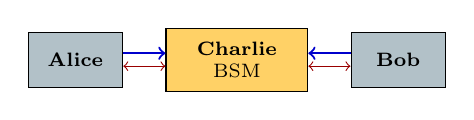
\begin{tikzpicture}[every node/.style={font=\scriptsize}, scale=0.82]
                \node[draw, fill=lightgray, minimum width=1.2cm, minimum height=0.7cm, align=center] (a) at (0,0) {\textbf{Alice}};
                \node[draw, fill=lightorange, minimum width=1.8cm, minimum height=0.8cm, align=center] (c) at (2.5,0) {\textbf{Charlie}\\BSM};
                \node[draw, fill=lightgray, minimum width=1.2cm, minimum height=0.7cm, align=center] (b) at (5.0,0) {\textbf{Bob}};
                \draw[->, blue!80!black, thick] ([yshift=0.1cm]a.east) -- ([yshift=0.1cm]c.west);
                \draw[->, blue!80!black, thick] ([yshift=0.1cm]b.west) -- ([yshift=0.1cm]c.east);
                \draw[<->, red!60!black] ([yshift=-0.1cm]a.east) -- ([yshift=-0.1cm]c.west);
                \draw[<->, red!60!black] ([yshift=-0.1cm]b.west) -- ([yshift=-0.1cm]c.east);
            \end{tikzpicture}
            \end{center}
        \end{column}
    \end{columns}

    \vspace{0.8cm}
    \small \textbf{Question:} how do device parameters propagate?
\end{frame}

% ── METHODOLOGY ───────────────────────────────────────────────────────────────
\begin{frame}{Methodology: Layered Physical Modelling}
    \textbf{Cumulative build-up}: isolates parameter contribution

    \vspace{0.08cm}
    \renewcommand{\arraystretch}{1.2}
    \scriptsize
    \begin{center}
    \begin{tabularx}{0.8\linewidth}{c>{\raggedright\arraybackslash}Xl}
        \toprule
        \textbf{Layer} & \textbf{Adds} & \textbf{Param.} \\
        \midrule
        0 & Ideal baseline               & — \\
        \lighthline
        1 & Fibre loss                   & $\alpha$ \\
        \lighthline
        2 & Detector efficiency          & $\eta_d$ \\
        \lighthline
        3 & Dark count rate              & $d_c$ \\
        \lighthline
        4 & TX insertion loss            & $L_i$ \\
        \lighthline
        5 & RX node/connector loss       & $L_n$ \\
        \lighthline
        6 & Source error rate            & $\varepsilon_s$ \\
        \lighthline
        7 & Fibre dephasing              & $\beta$ \\
        \lighthline
        8 & Beam splitter eff.\ (MDI)    & $\eta_{bs}$ \\
        \lighthline
        9 & Relay position (MDI)         & $d_{AC}/L$ \\
        \bottomrule
    \end{tabularx}
    \end{center}
    \normalsize
    \vspace{0.12cm}
    \texttt{Protocol} logic stays fixed between layers
\end{frame}

% ── CAPABILITY: P2P ───────────────────────────────────────────────────────────
\begin{frame}{NetSquid in Action: P2P Parameter Sweeps}
    \small 10 physical parameters swept over realistic ranges

    \vspace{0.05cm}
    \begin{center}
    \renewcommand{\arraystretch}{1.3}
    \setlength{\tabcolsep}{4pt}
    \tiny
    \begin{tabular}{llll}
        \toprule
        \textbf{Parameter} & \textbf{BB84} & \textbf{MDI} & \textbf{Why} \\
        \midrule
        Distance                & Log-Linear $\downarrow$           & Same slope, lower  & Total fibre loss identical; same exponential decay \\\lighthline
        Detector eff.\ $\eta_d$ & \textbf{Log-Linear} $\downarrow$  & \textbf{Log-Quadratic} $\downarrow$ & MDI coincidence requires both photons detected \\\lighthline
        Node/connector loss     & Log-Linear $\downarrow$           & 2x steeper $\downarrow$                   & Both arms lose independently; $(1-p)^2$ vs $(1-p)$ \\\lighthline
        Charlie placement       & N/A                           & Peaks at midpoint          & Symmetric arms optimise per-photon channel loss \\
        \bottomrule
    \end{tabular}
    \end{center}

    \vspace{0.1cm}
    \scriptsize \textbf{NetSquid:} $\eta_d^2$ MDI dependence emerges
    from simulation, new noise combinations predictable

    \vspace{0.25cm}
    \begin{columns}[T]
        \begin{column}{0.48\textwidth}
            \setlength{\fboxsep}{0pt}
            \setlength{\fboxrule}{0.6pt}
            \fcolorbox{blue!20!black}{white}{
\includegraphics[width=0.94\linewidth]{artefacts/img/efficiency.png}}
        \end{column}
        \begin{column}{0.48\textwidth}
            \setlength{\fboxsep}{0pt}
            \setlength{\fboxrule}{0.6pt}
            \fcolorbox{blue!20!black}{white}{
\includegraphics[width=\linewidth]{artefacts/img/charlie_pos.png}}
        \end{column}
    \end{columns}
\end{frame}

% ── NETWORK METHODOLOGIES ─────────────────────────────────────────────────────
\begin{frame}{Network Methodologies}
    \vspace{0.08cm}
    \setlength{\fboxsep}{0pt}\setlength{\fboxrule}{0.6pt}
    \fcolorbox{blue!20!black}{white}{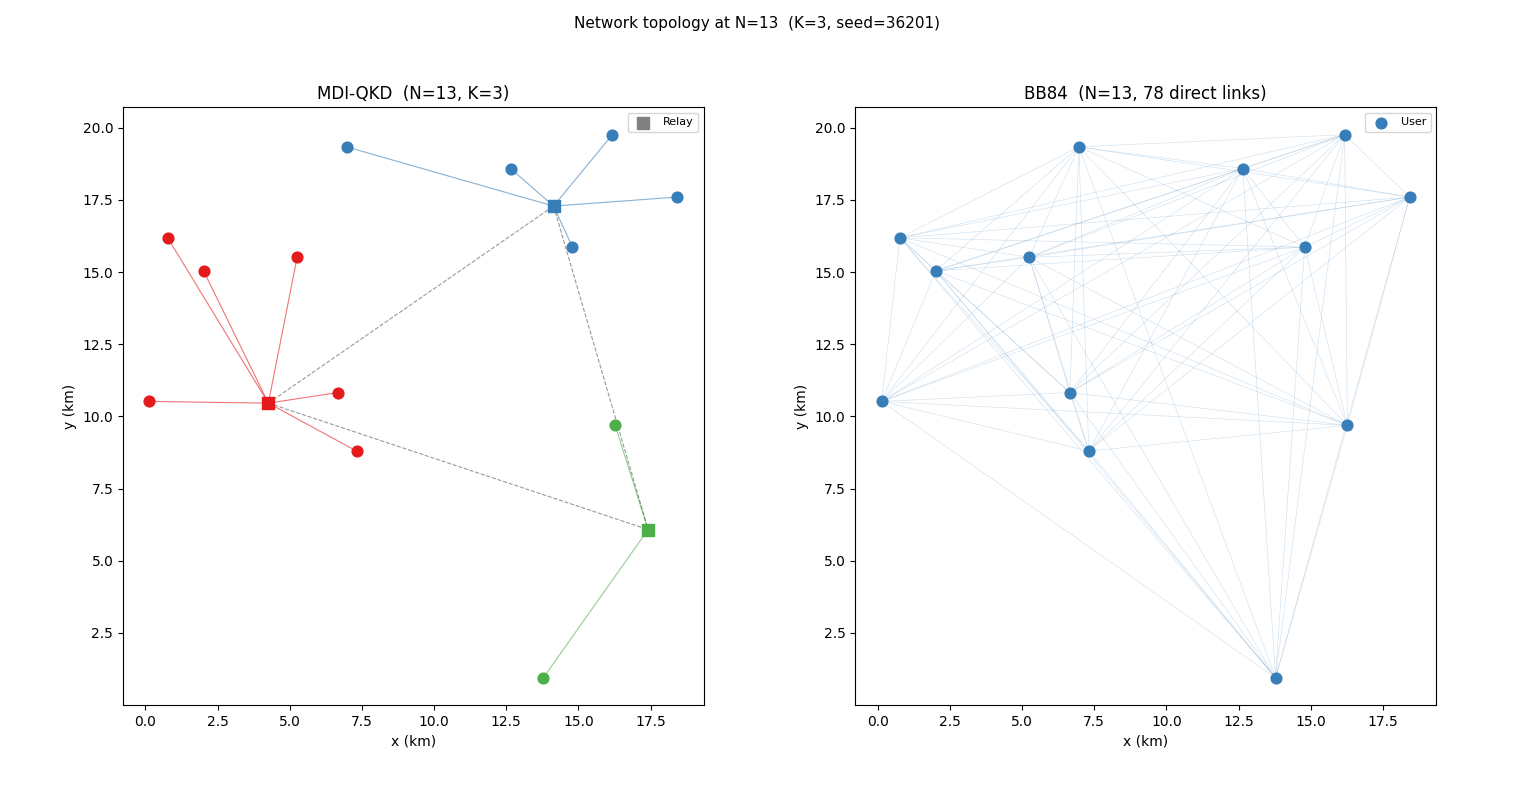
\includegraphics[width=0.95\linewidth]{artefacts/img/network_topology_viz.png}}

    \vspace{0.02cm}
    \tiny N=13 users, K=3 relays — MDI star topology (left) vs BB84 full mesh (right)

    \vspace{0.1cm}
    \begin{columns}[T]
        \begin{column}{0.50\textwidth}
            \textbf{\footnotesize MDI-QKD \& Trusted-node BB84}
            \begin{itemize}\scriptsize
                \item Star-mesh topology
                \item Cross-cluster pairs via relay mesh
                \item TN-BB84: \textbf{trusted} relay XORs keys
            \end{itemize}
        \end{column}
        \begin{column}{0.48\textwidth}
            \textbf{\footnotesize BB84, full mesh}
            \begin{itemize}\scriptsize
                \item Direct P2P link per user pair
                \item O($N^2$) fibre links
                \item Higher key rate
            \end{itemize}
        \end{column}
    \end{columns}
\end{frame}

% ── NETWORK SCALE RESULTS ─────────────────────────────────────────────────────
\begin{frame}{NetSquid in Action: Network Scale Results}
    \small Key rate swept over relay count $K$ and user count $N$ (multiple random seeds)

    \vspace{0.2cm}
    \begin{columns}[T]
        \begin{column}{0.48\textwidth}
            \setlength{\fboxsep}{0pt}\setlength{\fboxrule}{0.6pt}
            \fcolorbox{blue!20!black}{white}{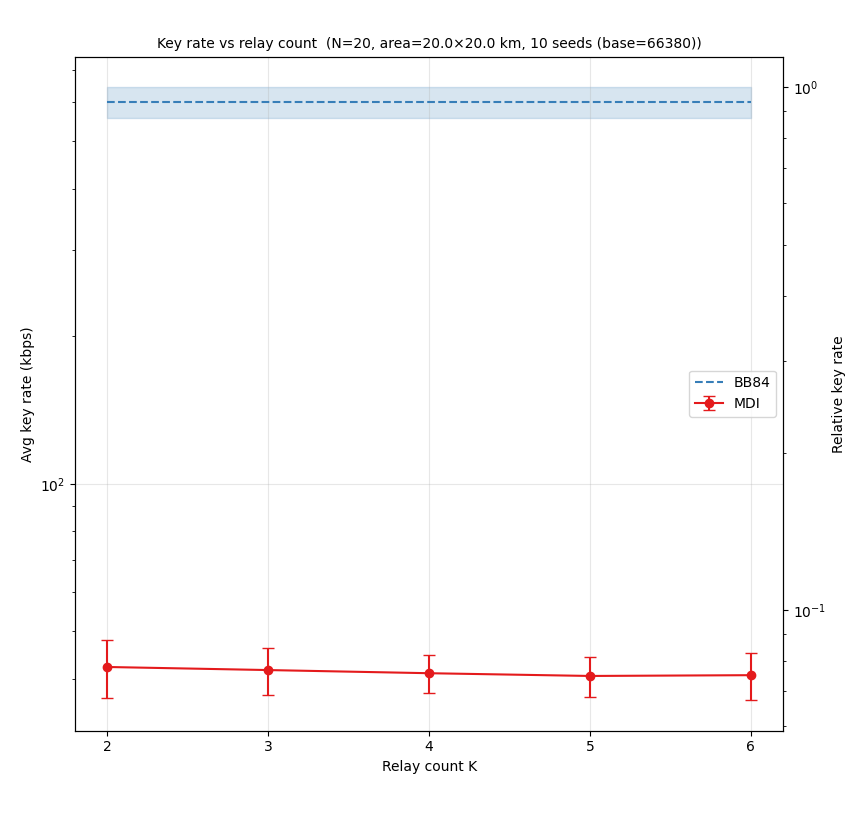
\includegraphics[width=0.94\linewidth]{artefacts/img/network_relay_count_20_users.png}}
        \end{column}
        \begin{column}{0.48\textwidth}
            \setlength{\fboxsep}{0pt}\setlength{\fboxrule}{0.6pt}
            \fcolorbox{blue!20!black}{white}{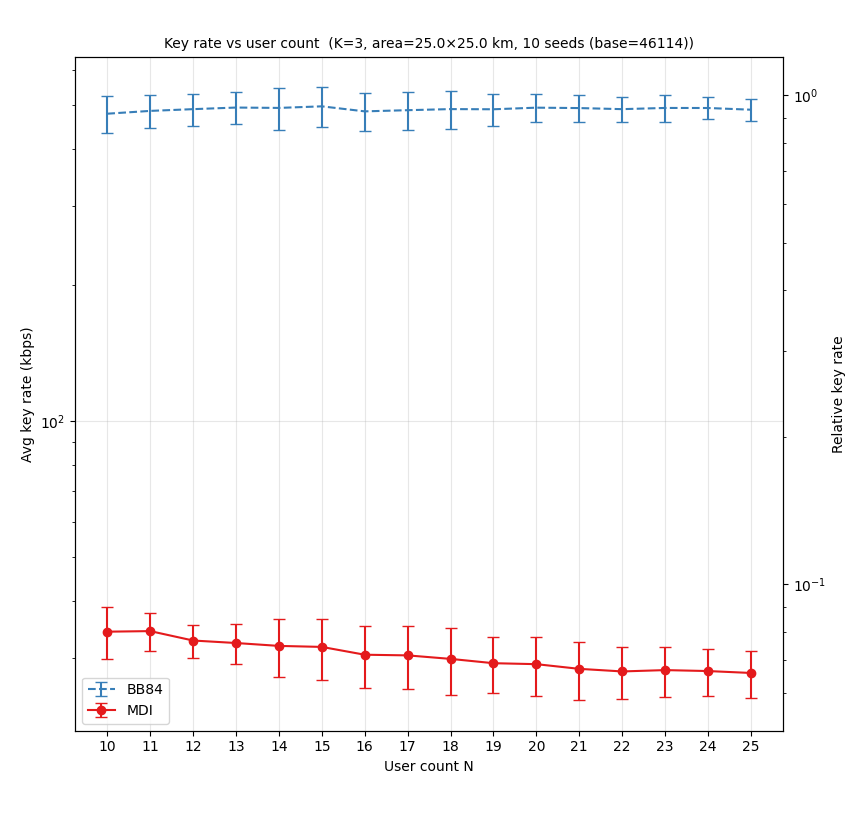
\includegraphics[width=0.94\linewidth]{artefacts/img/network_user_count_10_to_25.png}}
        \end{column}
    \end{columns}

    \vspace{0.15cm}
    \scriptsize MDI sits ${\sim}10\times$ below BB84 throughout, worse than P2P
\end{frame}

% ── BOTTLENECK: COMPUTE ───────────────────────────────────────────────────────
\begin{frame}{Bottleneck: Computational Cost}
    \textbf{NetSquid scales poorly with network size} (cf.\ Bel \textit{et al.}, 2024)

    \vspace{0.2cm}
    \begin{columns}[c]
        \begin{column}{0.48\textwidth}
            \renewcommand{\arraystretch}{1.7}
            \setlength{\tabcolsep}{3pt}
            \setlength{\aboverulesep}{0pt}
            \setlength{\belowrulesep}{0pt}
            \scriptsize
            \begin{tabular}{lrl}
                \toprule
                \textbf{Scenario} & \textbf{Time} & \\
                \midrule
                P2P sweep
                    & $\sim$min
                    & \textcolor{darkGreen}{\textbf{OK}} \\
                \lighthline
                $N{=}20$ relay sweep
                    & $\sim$hrs
                    & \textcolor{orange!80!black}{\textbf{Marginal}} \\
                \lighthline
                $N{=}100$ sweep
                    & $\sim$weeks
                    & \textcolor{red!70!black}{\textbf{Infeasible}} \\
                \bottomrule
            \end{tabular}
        \end{column}
        \begin{column}{0.52\textwidth}
            \setlength{\fboxsep}{0pt}\setlength{\fboxrule}{0.6pt}
            \fcolorbox{blue!20!black}{white}{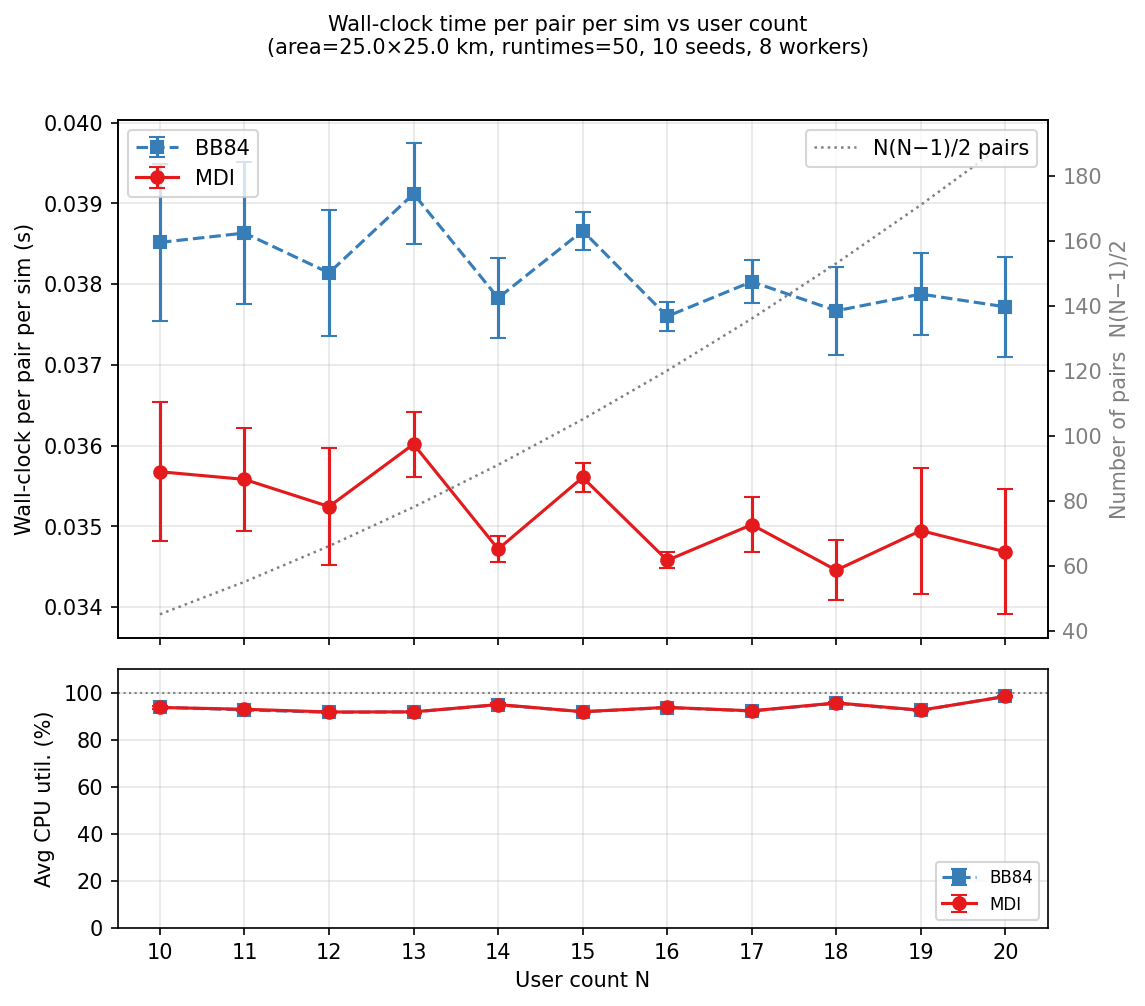
\includegraphics[width=0.9\columnwidth]{../../figures/July/17Jul26-overnight/time_vs_users.png}}
        \end{column}
    \end{columns}

    \vspace{0.15cm}
    \footnotesize \textbf{Root cause:} sequential event loop $\times$ $O(N^2)$ pairs $\times$ \texttt{spawn} overheads

    \vspace{0.08cm}
    \textbf{Note:} quantum state processing Netsquid's largest generic bottleneck
\end{frame}

% ── BOTTLENECK: PATHS FORWARD ─────────────────────────────────────────────────
\begin{frame}{Possible Directions}
    \vspace{0.15cm}
    \small Five levers from classical simulation; state compression quantum-native.

    \vspace{0.2cm}
    {\fontsize{6}{8}\selectfont
    \setlength{\tabcolsep}{5pt}
    \renewcommand{\arraystretch}{1.55}
    \begin{tabular}{@{}
        >{\raggedright\arraybackslash}p{2.3cm}
        >{\raggedright\arraybackslash}p{3.55cm}
        >{\raggedright\arraybackslash}p{3.55cm}@{}}
        \toprule
        \scriptsize\textbf{Strategy} & \scriptsize\textbf{Pro} & \scriptsize\textbf{Con} \\
        \midrule
        Distributed compute & Horizontal scaling; no fidelity cost & Entanglement breaks event-loop partitioning \\
        \lighthline
        Fluid/flow abstraction & Event count collapses & Analytic models topology-specific \\
        \lighthline
        State compression & Cheaper per event; exact within class & Restricted class; degrades outside \\
        \lighthline
        Surrogate modelling \textit{(tested)} & GP on coarse sim; dense grid evaluated instantly & Requires training; empirical validity \\
        \lighthline
        Engine optimisation & Zero fidelity cost & Gains limited by topology regularity \\
        \lighthline
        Adaptive sampling \textit{(tested)} & 30\% wall-clock saving (BB84) & Spawn overhead blocks MDI gain \\
        \bottomrule
    \end{tabular}
    }
\end{frame}

% ── ADAPTIVE MC: FINDINGS ─────────────────────────────────────────────────────
\begin{frame}{Adaptive Sampling: Protocol-Dependent Results}
    \small \textbf{Hypothesis:} stop MC once stable; use full budget for slow convergence

    \vspace{0.3cm}
    \begin{columns}[T]
        \begin{column}{0.42\textwidth}
            \renewcommand{\arraystretch}{1.35}
            \setlength{\tabcolsep}{4pt}
            \fontsize{6}{8}\selectfont
            \begin{tabular}{lccc}
                \toprule
                & \textbf{Run saving} & \textbf{Wall-clock} & \textbf{Rel.\ error} \\
                \midrule
                BB84 & 28\% & \textcolor{darkGreen}{\textbf{+30\%}} & <1\% \\
                MDI  & 0\%  & \textcolor{red!70!black}{$\approx 0\%$} & 2\% \\
                \bottomrule
            \end{tabular}

            \vspace{0.15cm}
            \textbf{\scriptsize BB84}
            \begin{itemize}\scriptsize
                \item Converges early
                \item Beyond cutoff, uses full budget
                \item Time savings at little penalty
            \end{itemize}

            \vspace{0.1cm}
            \textbf{\scriptsize MDI — never converges early}
            \begin{itemize}\scriptsize
                \item Structurally higher variance
                \item Requires in-loop sampling
            \end{itemize}
        \end{column}
        \begin{column}{0.56\textwidth}
            \hspace{-0.4cm}\fbox{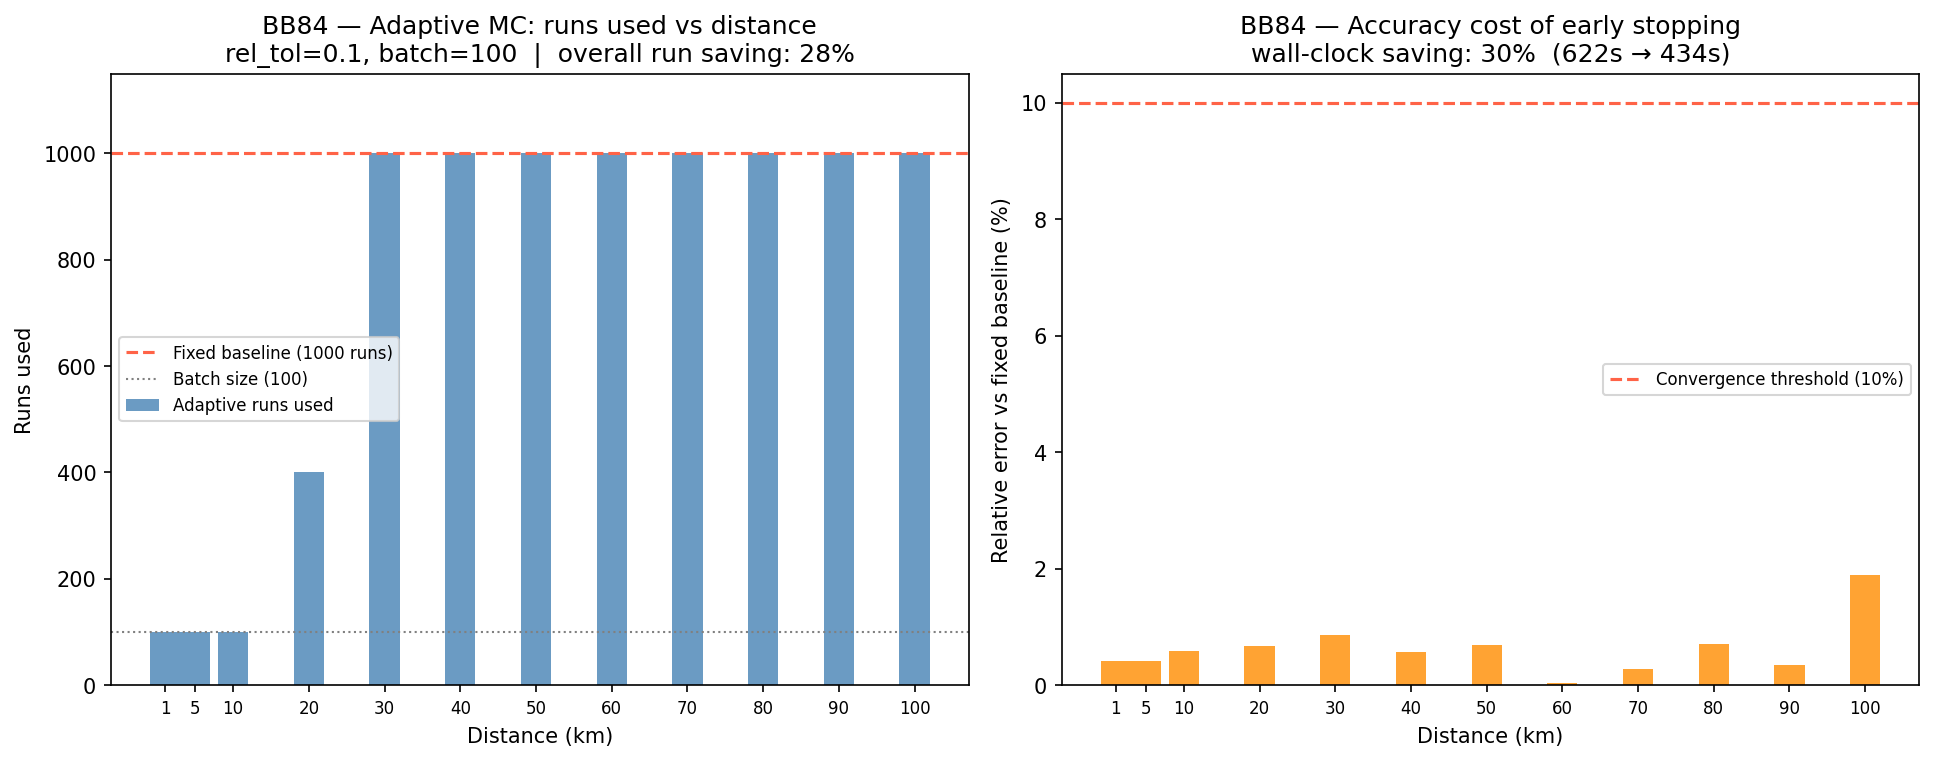
\includegraphics[width=1.02\columnwidth]{../../figures/July/17Jul26-overnight/adaptive_mc_bb84.png}}

            \vspace{0.4cm}
            \hspace{-0.4cm}\fbox{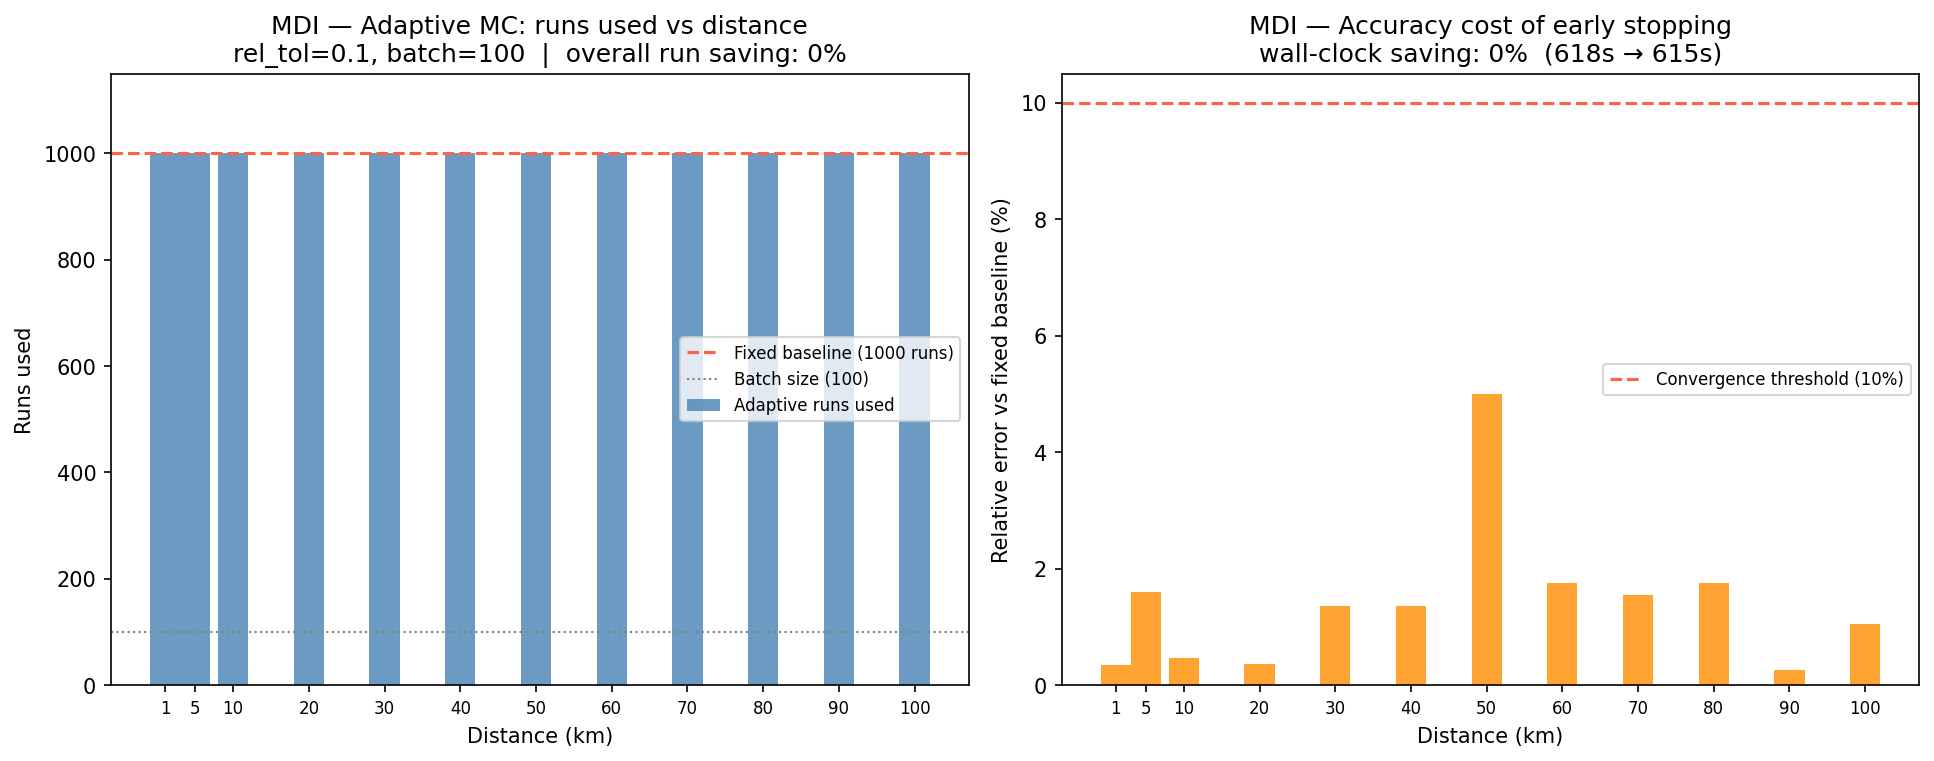
\includegraphics[width=1.02\columnwidth]{../../figures/July/17Jul26-overnight/adaptive_mc_mdi.png}}
        \end{column}
    \end{columns}
\end{frame}

% ── GP SURROGATE: PRELIMINARY RESULTS ────────────────────────────────────────
\begin{frame}{Surrogate Modelling: Preliminary Results}
    \textbf{GP trained on sims; predicts 10,000-point grid in $<$100\,ms}

    \vspace{0.3cm}
    \begin{columns}[T]
        \begin{column}{0.44\textwidth}
            \textbf{\scriptsize Speedup}
            \begin{itemize}\scriptsize
              \item \textbf{Linearly scaling speedup}
              \item Returns uncertainty at each data point by default (right panel)
              \item Interpolate over arbitrary conditions
              \item Trained once; re-evaluated instantly for any optimisation
            \end{itemize}

            \vspace{0.1cm}
            \textbf{\scriptsize Limitations}
            \begin{itemize}\scriptsize
                \item Large training requirement
                \item Extrapolation unreliable outside training range
                \item Doesn't solve the problem...
            \end{itemize}
        \end{column}
        \begin{column}{0.56\textwidth}
            \fbox{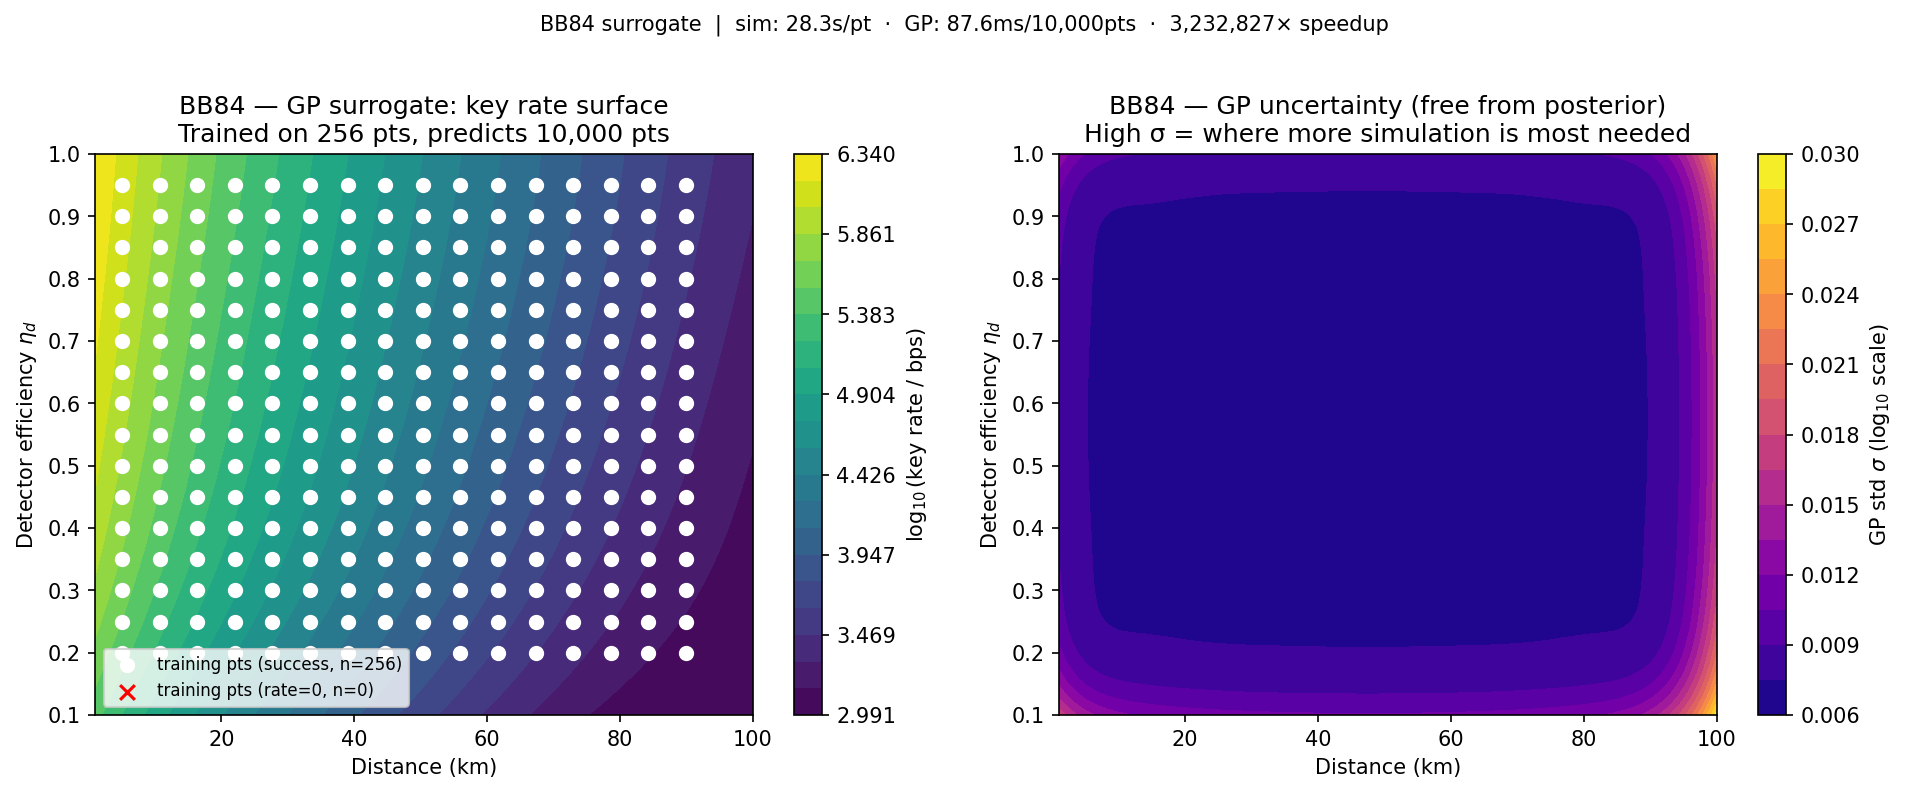
\includegraphics[width=0.94\columnwidth]{../../figures/July/17Jul26-overnight/surrogate_bb84.png}}

            \vspace{0.4cm}
            \fbox{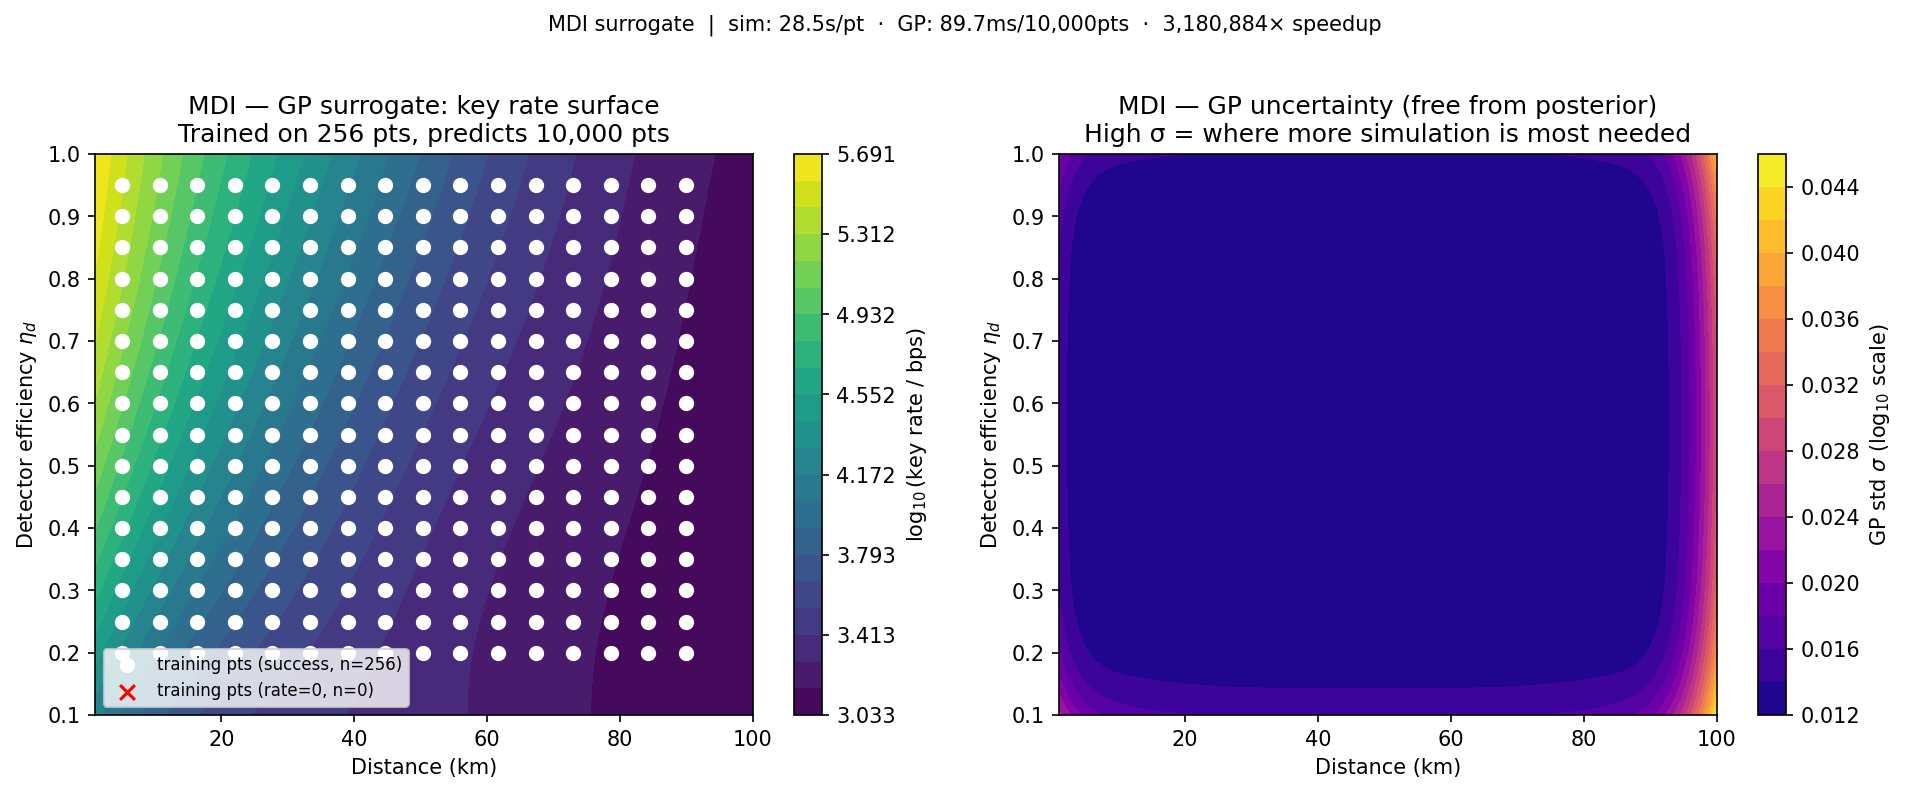
\includegraphics[width=0.94\columnwidth]{../../figures/July/17Jul26-overnight/surrogate_mdi.png}}
        \end{column}
    \end{columns}
\end{frame}

% ── FURTHER LIMITATIONS ───────────────────────────────────────────────────────
\begin{frame}{Further Limitations}
    QKD simulation engine limited beyond resource allocation

    \vspace{0.3cm}
    \begin{columns}[T]
        \begin{column}{0.48\textwidth}
            \textbf{Statistical}
            \begin{itemize}\scriptsize
                \item High MC variance near QBER cutoff
                \item Asymptotic key rate only
                \item Block size limit $n{=}1024$; finite-key penalty unquantified
            \end{itemize}
        \end{column}
        \begin{column}{0.48\textwidth}
            \textbf{Protocol}
            \begin{itemize}\scriptsize
                \item Ideal sifting - no EC or PA overhead simulated
                \item Timing jitter/synchronicity not modelled
                \item Ideal single-photon source throughout
            \end{itemize}
        \end{column}
    \end{columns}

    \vspace{0.4cm}
    \begin{columns}[T]
        \begin{column}{0.48\textwidth}
            \textbf{Network}
            \begin{itemize}\scriptsize
                \item No multi-user scheduling or contention
                \item No WDM - single pair per relay at a time
                \item No quantum storage model
            \end{itemize}
        \end{column}
        \begin{column}{0.48\textwidth}
            \textbf{Validation}
            \begin{itemize}\scriptsize
                \item Benchmarked against limited catalogue of experimental data + PLOB
            \end{itemize}
        \end{column}
    \end{columns}
\end{frame}

% ── THE BIG QUESTION ──────────────────────────────────────────────────────────
\begin{frame}{Lessons and an Open Question}
    \textbf{What using NetSquid at this scale reveals:}

    \begin{itemize}\small
        \item DES is powerful at small scale - arbitrary and repeatable conditions
        \item Computationally intractable as user connectivity grows
        \item Causal event loop a \textbf{fundamental} constraint
    \end{itemize}

    \vspace{0.15cm}
    \setlength{\fboxsep}{8pt}\setlength{\fboxrule}{1.4pt}
    \fbox{\parbox{\dimexpr\linewidth-2\fboxsep-2\fboxrule\relax}{%
        \textcolor{orange!90!black}{\textbf{\textbf{Open question}}}\\[0.25cm]
        To \textbf{optimise} existing DES, or does quantum causal structure~demand~\textbf{bespoke} models \& simulation?%
    }}
\end{frame}

% ── SUMMARY ───────────────────────────────────────────────────────────────────
\begin{frame}{Summary}
    \begin{itemize}
        \item \textbf{NetSquid:} powerful DES framework for low-computation quantum network protocols
        \item \textbf{Demonstrated on BB84 vs MDI-QKD} at P2P and metropolitan network scale
        \item \textbf{Binding constraint:} computational cost, is DES the right abstraction?
    \end{itemize}

    \vspace{0.2cm}
    \begin{center}
        \large Thank you for listening!

        \vspace{0.1cm}
        \normalsize \textit{Supervised by Dr.\ Alejandra Beghelli \& Dr.\ Emilio Hugues-Salas (BT Group), organised by UCL Department of Physics \& Astronomy}
    \end{center}
\end{frame}

% ── BACKUP SLIDES ─────────────────────────────────────────────────────────────
\appendix

% ── BACKUP: GPU ───────────────────────────────────────────────────────────────
\begin{frame}{Backup: Why GPU Acceleration Does Not Help}
    \small A natural question: can the compute bottleneck be addressed with GPU parallelism?

    \vspace{0.2cm}
    \begin{columns}[T]
        \begin{column}{0.48\textwidth}
            \textbf{Where GPUs excel}
            \begin{itemize}\scriptsize
                \item Large batched linear algebra — density matrices of ${\geq}20$ qubits
                \item Tensor network contraction over many-body systems
                \item Training ML surrogates (not inference)
            \end{itemize}

            \vspace{0.2cm}
            \textbf{What this simulation does}
            \begin{itemize}\scriptsize
                \item BB84 / MDI operate on 1--2 qubits — density matrices are $2\times2$ or $4\times4$
                \item GPU overhead dominates; CPU is faster for operations this small
                \item NetSquid has no GPU backend — Python + C extensions, CPU-only
            \end{itemize}
        \end{column}
        \begin{column}{0.48\textwidth}
            \textbf{The real bottlenecks are architectural}
            \begin{itemize}\scriptsize
                \item \textbf{Sequential event loop:} events are causally ordered within each run —
                      cannot be parallelised on GPU or CPU
                \item \textbf{Spawn overhead:} each MC batch launches a new OS process;
                      ${\approx}2$--$3$\,s regardless of workload
                \item \textbf{O($N^2$) pair count:} the combinatorial scaling problem;
                      GPU arithmetic does not reduce pair count
            \end{itemize}

            \vspace{0.2cm}
            \begin{alertblock}{}
                \scriptsize The bottleneck is \textbf{control flow and process management},
                not floating-point throughput. GPU does not address either.
            \end{alertblock}
        \end{column}
    \end{columns}
\end{frame}

% ── BACKUP: EXTENSIONS ────────────────────────────────────────────────────────
\begin{frame}{Backup: What Else NetSquid Can Express}
    \small The same \texttt{Node} / \texttt{Protocol} / \texttt{Channel} structure extends naturally:

    \vspace{0.2cm}
    \begin{columns}[T]
        \begin{column}{0.47\textwidth}
            \textbf{Decoy-state QKD}
            \begin{itemize}\scriptsize
                \item Replace ideal single-photon source with WCP ($\mu$ signal, $\nu$ decoy, vacuum)
                \item Poisson-distributed photon number per pulse — NetSquid source model change
                \item Protocol layer estimates single-photon gain/QBER from decoy statistics
                \item Key rate formula updates to (Ma \textit{et al.}, 2005) decoy bound
                \item NetSquid captures pulse-by-pulse statistics naturally; no approximation needed for multi-intensity logic
            \end{itemize}
        \end{column}
        \begin{column}{0.50\textwidth}
            \textbf{Quantum repeater chain} \textnormal{\scriptsize (Coopmans \textit{et al.}, 2021)}
            \begin{center}
            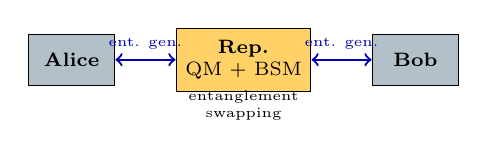
\begin{tikzpicture}[every node/.style={font=\scriptsize}, scale=0.78]
                \node[draw, fill=lightgray, minimum width=1.1cm, minimum height=0.65cm, align=center] (a) at (0,0) {\textbf{Alice}};
                \node[draw, fill=lightorange, minimum width=1.3cm, minimum height=0.8cm, align=center] (r) at (2.8,0) {\textbf{Rep.}\\QM + BSM};
                \node[draw, fill=lightgray, minimum width=1.1cm, minimum height=0.65cm, align=center] (b) at (5.6,0) {\textbf{Bob}};
                \draw[blue!70!black, thick, <->] (a) -- node[above]{\tiny ent. gen.} (r);
                \draw[blue!70!black, thick, <->] (r) -- node[above]{\tiny ent. gen.} (b);
                \node[font=\tiny, align=center] at (2.8,-0.75) {entanglement\\swapping};
            \end{tikzpicture}
            \end{center}
            \begin{itemize}\scriptsize
                \item Quantum memory at repeater holds entanglement while second link establishes
                \item BSM at repeater swaps entanglement end-to-end
                \item T\textsubscript{1}/T\textsubscript{2} decoherence captured by \texttt{QuantumMemory}
                \item Rate scales as $\eta_d^2$ per link, $\sim(\eta_d^2)^N$ across $N$ hops
            \end{itemize}
        \end{column}
    \end{columns}
\end{frame}

% ── BACKUP: METROPOLITAN NETWORK TOPOLOGY ─────────────────────────────────────
\begin{frame}{Backup: Metropolitan Network Topology}
    \begin{center}
    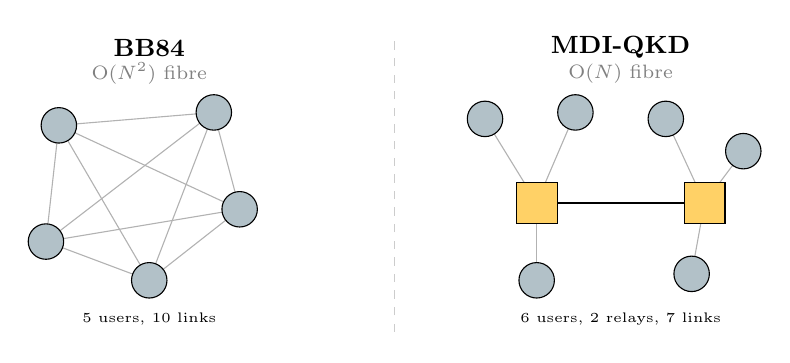
\begin{tikzpicture}[every node/.style={font=\tiny}, scale=0.82]

        % BB84 panel
        \node[font=\small\bfseries] at (-3.8, 2.6) {BB84};
        \node[font=\scriptsize, text=gray] at (-3.8, 2.2) {O($N^2$) fibre};

        \coordinate (u1) at (-5.2, 1.4);
        \coordinate (u2) at (-2.8, 1.6);
        \coordinate (u3) at (-2.4, 0.1);
        \coordinate (u4) at (-3.8,-1.0);
        \coordinate (u5) at (-5.4,-0.4);

        \foreach \a/\b in {u1/u2, u1/u3, u1/u4, u1/u5,
                            u2/u3, u2/u4, u2/u5,
                            u3/u4, u3/u5, u4/u5}{
            \draw[gray!60, thin] (\a) -- (\b);
        }
        \foreach \p in {u1,u2,u3,u4,u5}{
            \node[draw, circle, fill=lightgray, minimum size=0.45cm] at (\p) {};
        }
        \node[font=\tiny] at (-3.8,-1.6) {5 users, 10 links};

        \draw[gray!40, dashed] (0,-1.8) -- (0,2.8);

        % MDI panel
        \node[font=\small\bfseries] at (3.5, 2.6) {MDI-QKD};
        \node[font=\scriptsize, text=gray] at (3.5, 2.2) {O($N$) fibre};

        \coordinate (r1) at (2.2, 0.2);
        \coordinate (r2) at (4.8, 0.2);
        \draw[black, thick] (r1) -- (r2);

        \coordinate (v1) at (1.4, 1.5);
        \coordinate (v2) at (2.8, 1.6);
        \coordinate (v3) at (4.2, 1.5);
        \coordinate (v4) at (5.4, 1.0);
        \coordinate (v5) at (4.6,-0.9);
        \coordinate (v6) at (2.2,-1.0);

        \foreach \v in {v1,v2,v6}{ \draw[gray!60, thin] (\v) -- (r1); }
        \foreach \v in {v3,v4,v5}{ \draw[gray!60, thin] (\v) -- (r2); }

        \foreach \p in {v1,v2,v3,v4,v5,v6}{
            \node[draw, circle, fill=lightgray, minimum size=0.45cm] at (\p) {};
        }
        \foreach \r in {r1,r2}{
            \node[draw, rectangle, fill=lightorange, minimum size=0.52cm] at (\r) {};
        }
        \node[font=\tiny] at (3.5,-1.6) {6 users, 2 relays, 7 links};

    \end{tikzpicture}
    \end{center}

    \vspace{-0.1cm}
    \scriptsize
    Relay placement: k-means, minimising total user-to-relay distance.
    Cross-cluster MDI pairs re-routed passively via optical switch (1 dB insertion loss).
    \textbf{Key finding:} BB84 outperforms MDI more severely at network scale (${\sim}10\times$)
    than at P2P (${\sim}3\times$) — cause under investigation.
\end{frame}

\begin{frame}{Backup: Physical Parameter Reference}
    \renewcommand{\arraystretch}{1.3}
    \scriptsize
    \begin{tabular}{llll}
        \toprule
        \textbf{Parameter} & \textbf{Symbol} & \textbf{Realistic range} & \textbf{Typical value} \\
        \midrule
        Distance              & $L$             & 5--50 km              & 20 km (metropolitan) \\
        \lighthline
        Fibre loss            & $\alpha$        & 0.15--0.25 dB/km      & 0.20 dB/km (SMF-28) \\
        \lighthline
        Detector efficiency   & $\eta_d$        & 0.15--0.95            & 0.65 (SNSPD) \\
        \lighthline
        Dark count rate       & $d_c$           & 1--10{,}000 cps       & 100 cps (SNSPD) \\
        \lighthline
        TX insertion loss     & $L_i$           & 2--20\%               & 10\% \\
        \lighthline
        RX node loss          & $L_n$           & 0.5--4 dB             & 2 dB \\
        \lighthline
        Source error rate     & $\varepsilon_s$ & 0.1--2\%              & 0.5\% \\
        \lighthline
        Fibre dephasing       & $\beta$         & $2.6\times10^{-7}$--$3.8\times10^{-7}$/km & $3.2\times10^{-7}$/km \\
        \lighthline
        Beam splitter eff.    & $\eta_{bs}$     & 0.90--0.99            & 0.97 \\
        \bottomrule
    \end{tabular}
\end{frame}

\begin{frame}{Backup: Monte Carlo Methodology}
    \textbf{Why Monte Carlo?}
    \begin{itemize}\small
        \item Single deterministic run insufficient — stochastic loss, basis choice, dark counts
        \item 100 runs per sweep point gives distribution of key rates
        \item Report mean $\pm\,\sigma$; min/max whiskers on select plots
    \end{itemize}

    \vspace{0.2cm}
    \textbf{Known statistical issues}
    \begin{itemize}\small
        \item At high loss / long distance, most runs produce no key (QBER $> 11\%$)
        \item Failed runs excluded before aggregation $\to$ surviving runs cluster near threshold;
              lower error bars absent in high-loss regime — artefact of cutoff filtering
        \item Current default: 100 runs, 1024 photons per run;
              target ${\geq}1000$ runs for $<10\%$ relative error at low key rates
    \end{itemize}
\end{frame}

\begin{frame}{Backup: Infrastructure Scaling}
    \renewcommand{\arraystretch}{1.4}
    \scriptsize
    \begin{tabular}{lll}
        \toprule
        & \textbf{BB84} & \textbf{MDI-QKD} \\
        \midrule
        Fibre links     & $N(N-1)/2$ direct P2P     & $N$ user-relay; $K(K-1)/2$ relay-relay \\
        Relay hardware  & None                       & $K$ Charlie nodes (untrusted) \\
        Trust model     & Detector trusted           & Detector untrusted \\
        Infrastructure  & O($N^2$)                   & O($N$) \\
        \midrule
        Key rate gap    & Higher (P2P and network)   & Lower; gap widens at network scale \\
        \bottomrule
    \end{tabular}

    \vspace{0.3cm}
    \small At large $N$, MDI fibre cost grows far more slowly — the primary economic argument for
    network-scale MDI deployment despite the key rate penalty.
\end{frame}

\end{document}
